\section{Planning}
De planning voor de opdracht bij Getinge Applikon is te zien in figuur \ref{fig:planning}, de planning is weergegeven in een Gantt Chart. Voor mijn opdracht houd ik me bezig met het ontwerpen, produceren en testen van het systeem. In het tijdschema is het project opgedeeld in fases en opdrachten met een geschatte
looptijd. De vijf hoofdfases zijn: inlezen en onderzoek, Ontwerpen, Productie en test, software ontwikkeling en Compare Model. Elke fasen is opgedeeld in subtaken, het afronden van een fase zal worden gezien als een milestone. Voordat een milestone wordt afgerond zal het verslag worden bijgewerkt. De planning is onderhevig aan verandering en de Gantt Chart kan indien gewenst en nodig aangepast worden.

\begin{figure}[H]
	\centering
	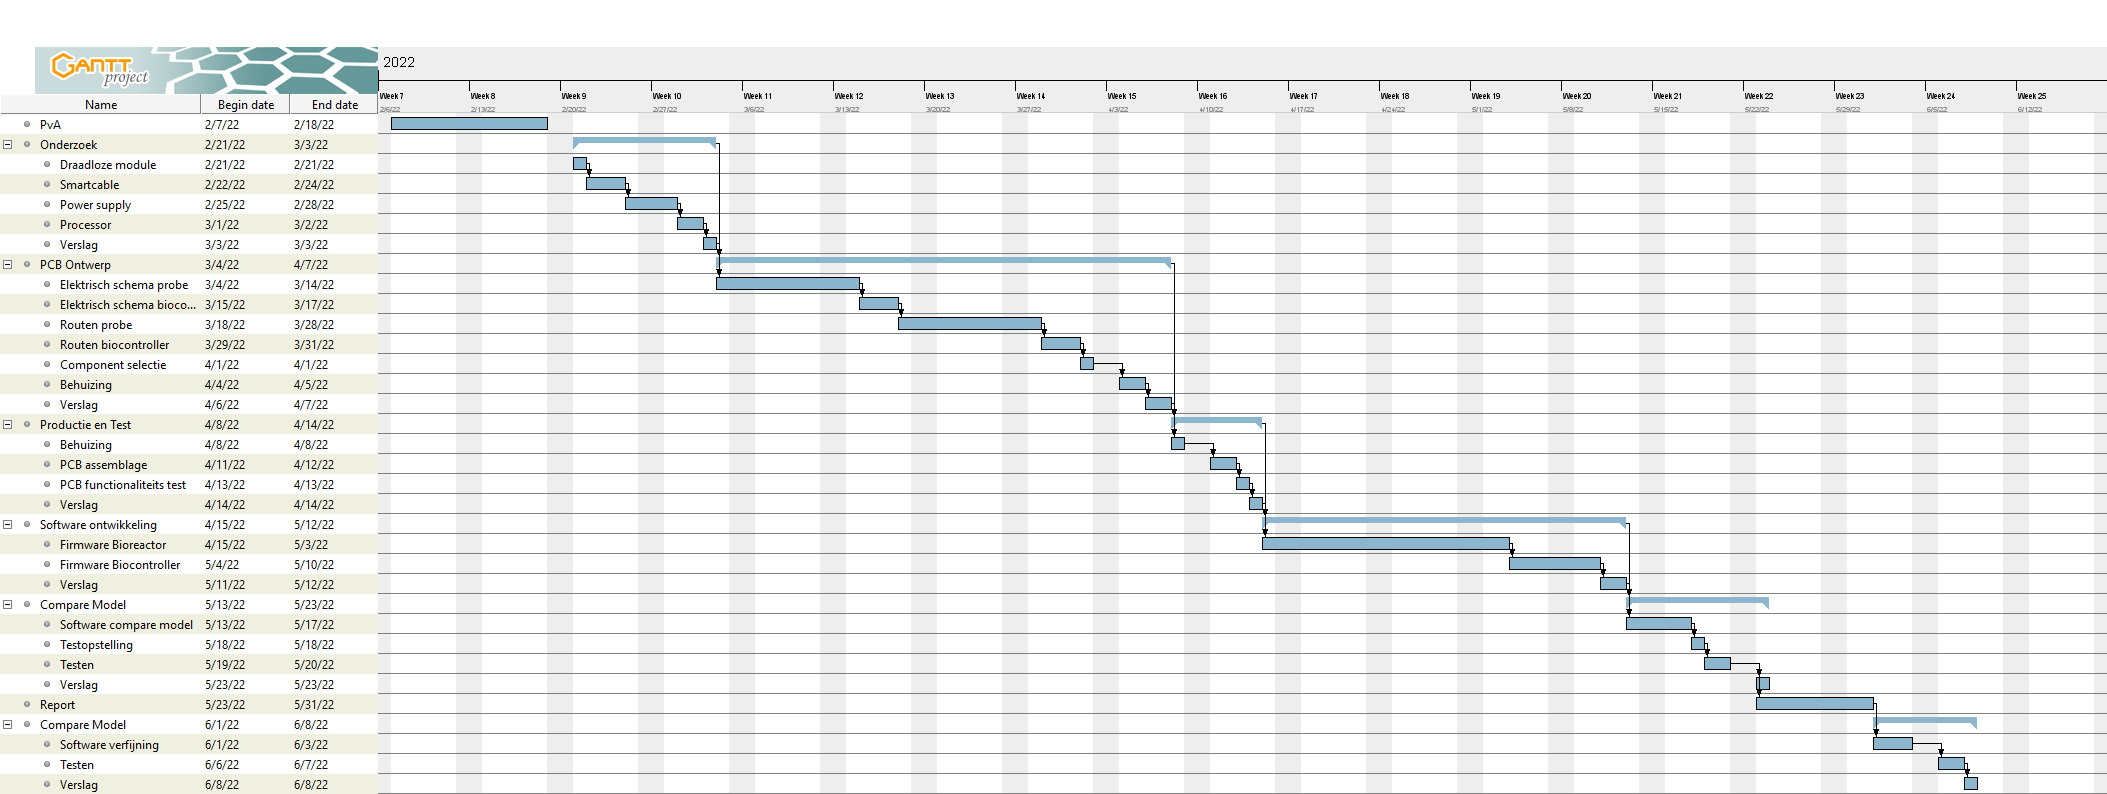
\includegraphics[width=1.0\linewidth]{graphics/planning_appl}
	\caption{Een Gantt-grafiek voor de stageperiode.}
	\label{fig:planning}
\end{figure}


